\documentclass[
	12pt, % Default font size, values between 10pt-12pt are allowed
	%letterpaper, % Uncomment for US letter paper size
	%spanish, % Uncomment for Spanish
]{refrigeration_report_style}

\usepackage{my_packages}
\usepackage{comment}
\usepackage[inkscapeformat=png]{svg}
\usepackage{subcaption}
\usepackage{multicol}
\usepackage[hidelinks,colorlinks=true,linkcolor=blue,citecolor=blue]{hyperref}
\usepackage[font=small,labelfont=bf]{caption}

%-------------- To Do: --------------------------------------------------------------
\begin{comment}
    - Fix SPECTRE acronym uses i.e. Supersonic Phase-change Ejecter Cycle --> SPEC
    - Read through for clarity and grammar
    - Input CO_2 data/graphs (MAKE IT WORK!!!)
\end{comment}
%------------------------------------------------------------------------------------

\title{Fluids Poject}        % Assignment title
\author{Authors by Last Name: Heath Buer, Joshua Hoffman, McCade Hughes, Bennet Outland, Joseph Romero}   % Student name
%Partner Name
%\roll{Lorem Ipsum, Lorem Ipsum}                    % Class roll
\class{Thermo Fluid Dynamics}              % Class
\session{M01}             % Session
\email{\\ heath.buer@mines.sdsmt.edu \\ joshua.hoffman@mines.sdsmt.edu \\  lane.hughes@mines.sdsmt.edu \\ bennet.outland@mines.sdsmt.edu \\ joseph.romero@mines.sdsmt.edu}
\date{May 2, 2023}% Due date
\institute{Department of Mechanical Engineering}              % Institute or school name
\course{ME 331}                            % Course or course name
\professor{Dr. John Thalakkottor}                                           % Professor or teacher in charge of the assignment

%------------------------------------------------------------------------------------
\addbibresource{ref.bib} 

\setcounter{secnumdepth}{-2} 
%\renewcommand{\thesection}{}  % https://tex.stackexchange.com/a/30202/114006
%------------------------------------------------------------------------------------
\begin{document}
\maketitle 
\begin{table}
    \centering
    \begin{tabular}{c|c}
        Name & \% Effort \\
        \hline
        Heath Buer & 100\% \\
        Joshua Hoffman & 100\% \\
        McCade Hughes & 100\% \\
        Bennet Outland & 100\% \\
        Joseph Romero & 100\%
    \end{tabular}
\end{table}





\pagenumbering{gobble}  
\newpage
\pdfbookmark[section]{\contentsname}{toc}
\tableofcontents
\newpage
\pagenumbering{arabic}          % to start the page numbering

%-----------------------------------------
%1 Significance, Design Requirements, and Objectives
\section{Summary}
\lipsum[1]

%2
\section{Introduction}
The goal of this project was to determine values for the coefficient of lift and drag for a Clark Y-14 Airfoil at different velocities and angles of attack. Those values were then used to determine the minimum required runway length for safe take-off and landing as well as the minimum thrust required for take-off given the max aircraft mass, airfoil type, wing span, wing aspect ratio, and factor of safety for runway length. 

%3
\section{Description of Apparatus}
One of the methods used for determining the $C_D$ was using pressure data from a wind tunnel experiment. The Clark Y-14 Airfoil was tested in the wind tunnel at 40mph, 65mph, and 90 mph. Pressure data was taken at angles of attack of 0, 5, 10, 15, and 20 degrees. The pressure data was taken using orifices in the airfoil surface connected to manometers. Height differences for each pressure port were taken in reference to a manometer connected to the atmosphere. These height differences were then used to calculate $C_D$. 

% Describe the math behind finding C_D and C_L using pressure data (trapezoidal rule etc.). 

%4
\section{Description of Numerical Simulation} 
\lipsum[1]
 
%5
\section{Results}


\subsection{Project Objective 1}
% plots outlined in the Objective 1 section of the assignment description. results for C_D and C_L for wind tunnel and CFD. 

\begin{figure}[H]% 
    \centering
    {{\includegraphics[width=10cm]{figures/C_L_vs_alpha.jpg} }}% 
    \caption{Plot of $C_L$ vs. $\alpha$ data from the wind tunnel experiment and CFD}
    \label{fig:C_L_vs_alpha}%
\end{figure}  

\begin{figure}[H]% 
    \centering
    {{\includegraphics[width=10cm]{figures/C_D_vs_alpha.jpg} }}% 
    \caption{Plot of $C_D$ vs. $\alpha$ data from the wind tunnel experiment and CFD.}
    \label{fig:C_D_vs_alpha}%
\end{figure}  

\begin{figure}[H]% 
    \centering
    {{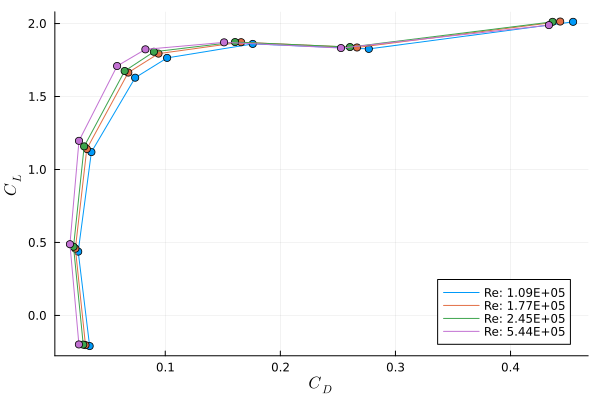
\includegraphics[width=10cm]{figures/C_L_C_D_vs_alpha.jpg} }}% 
    \caption{Plot of $C_L$ vs. $\alpha$ data from the wind tunnel experiment and CFD.}
    \label{fig:C_L_C_D_vs_alpha}%
\end{figure}  

\begin{figure}[H]% 
    \centering
    {{\includegraphics[width=10cm]{figures/C_L_vs_C_D.jpg} }}% 
    \caption{Plots of $C_L$ vs. $\alpha$ data from the wind tunnel experiment and CFD.}
    \label{fig:C_L_vs_C_D}%
\end{figure}  

\subsection{Project Objective 2}
The minimum necessary runway length was calculated for the plane to safely land. The sum of forces in the Y produced the following equation for velocity.

\begin{align*}
    V = \sqrt{\frac{2mg}{C_{L}\rho A}} \\
\end{align*}

\noindent This velocity at touchdown is a function of $C_L$ which varies with velocity. In order to fix this problem, a guess and check method was used to find the $C_L$ value at which the velocity produced by our equations matched the velocity at that $C_L$. Values for $C_L$ in between data were approximated using linear approximation. 

\par
\bigskip

\noindent Deceleration due to drag, $C_D$, and $C_L$ were assumed to be constant for the entire duration of landing and taking off. Using kinematic equations for constant acceleration the minimum length of the runway was determined to be 

\begin{align*}
    x = \frac{-V_{i}^{2}}{2a} \\
\end{align*}

\noindent Using the sum of forces in the X direction 

\begin{align*}
    a = \frac{-F_{D}}{m} \\
\end{align*}

\noindent Substituting and simplifying yields the result

\begin{equation}
    x = \frac{m}{C_{D}\rho A} 
    \label{eq:x} \\
\end{equation}
\vspace{2mm}

\noindent Velocity for liftoff was assumed to be equivalent to the initial velocity during landing. This assumption, along with the sum of forces in the X direction produced the following equation for the minimum force of thrust.

\begin{equation}
    F_{t} = \frac{mV^2}{2x} + \frac{C_{D} \rho V^2 A}{2} 
    \label{eq:F_t} \\
\end{equation}


Equations (\ref{eq:x}) and (\ref{eq:F_t}) yield a runway length of ????? and a minimum thrust of ?????. With a factor of safety incorporated the length of the runway will be ?????.  

%6
\section{Discussion}
\lipsum[1]

% analysis of different results of wind tunnel and CFD and which results are used with justification. 

% Analysis of runway length and thrust and discussion on the reliability of our results. 


\section{Appendices}


\par
\bigskip

\newpage
\phantomsection   % 
\printbibliography[heading=bibintoc, title={References}]

\begin{comment}
\newpage
\section{Appendix}
\indent
\lipsum[1]
\end{comment}

\end{document}

